\documentclass[11pt,a4paper]{article}
\usepackage[T1]{fontenc}
\usepackage[margin=2.3cm]{geometry}
\usepackage{amsmath,amssymb}
\usepackage{graphicx}
\usepackage[dvipsnames]{xcolor}
\usepackage{enumitem}
\usepackage[colorlinks=true,linkcolor=blue,urlcolor=blue]{hyperref}
\setlength{\parskip}{0.6em}
\setlength{\parindent}{0pt}
\begin{document}

\begin{center}{\LARGE\bfseries opensolidmodel}\\[0.4em]{\large Learn how a parametric CAD program stores, rebuilds and measures a part, in three sessions.}\\[0.2em]\small PAN IIT OSS explainer \textbullet{} diploma/undergrad to advanced undergrad (levels 2-4)\end{center}

\section*{Why this exists}
Every manufactured part started as a CAD model, and a good model changes when the requirements change. This explainer shows the mathematics inside: named parameters with equations, the properties of a profile and a solver that keeps a sketch consistent, which you can build yourself.

\section*{The end goal}
The end goal is to build a small parametric CAD kernel like SolidWorks. The same ideas carry over to the feature tree, the sketch solver and the geometry engine of a full CAD program, which use many more feature types and careful handling of curves and surfaces.

\section*{How the three sessions build up}
\begin{enumerate}[nosep]
\item \textbf{Session 1: A part is a recipe, not a shape: parameters, equations and a rebuild} (Level 2: mathematical engineering model, 60 min).
\item \textbf{Session 2: From an outline to the properties of a solid: area, centroid and stiffness} (Level 3: simulation and validation, 75 min).
\item \textbf{Session 3: How a sketch keeps its corners where you told it: a constraint solver} (Level 3: simulation and validation, 75 min).
\end{enumerate}

\section{Session 1: A part is a recipe, not a shape: parameters, equations and a rebuild}

\subsection*{A. Real-world problem}
A customer asks for the same mounting plate with 6 holes instead of 4, and 20 mm wider. In a drawing you would redraw it. A CAD program stores a recipe instead and rebuilds the part when one number changes. How is such a recipe stored, and how do we get the volume and the mass of the rebuilt part? The plate in this repo is 120 x 40 x 8 mm steel with 4 holes: how much does it weigh, and what happens to the weight when the customer's change is made?

\subsection*{B. Concept and theory}
A parametric part is stored as three things. First, a dictionary of named parameters (width w, depth d, thickness h, number of holes n, hole ratio). Second, a list of equations that compute other dimensions from the parameters, for example the hole spacing s = w / (n + 1) and the hole diameter dia = ratio x s; these are stored as text and evaluated with the current values. Third, a list of features applied in order: a block w x d x h, then n round through-holes of diameter dia in a row, s apart. To rebuild, we change the parameters, evaluate the equations in order (a later equation may use an earlier one), check that the recipe still makes sense (the holes must not touch each other or the edges), and recompute the geometry. For this plate the volume is the block minus the holes, V = w d h - n (pi / 4) dia\textasciicircum{}2 h, and the mass is the density times the volume, with rho = 7850 kg/m\textasciicircum{}3 for steel. Because the diameter is tied to the spacing, a change of w or n moves every hole and resizes it. The equation evaluator must never run arbitrary code, because a recipe can come from another person: it accepts only numbers, names, + - * / **, brackets and a short list of functions, and refuses everything else, including huge powers that would hang the program.

\begin{itemize}[nosep]
\item w, d, h: width, depth and thickness of the plate (mm)
\item n: number of holes (a whole number) (no unit)
\item ratio: hole diameter as a fraction of the hole spacing (no unit)
\item s: hole spacing, w / (n + 1) (mm)
\item dia: hole diameter, ratio x s (mm)
\item V: volume of the plate with its holes (mm\textasciicircum{}3)
\item rho: density of steel (kg/m\textasciicircum{}3 (7850))
\end{itemize}

\[ s = \frac{w}{n + 1},\qquad \mathrm{dia} = \mathrm{ratio}\cdot s \]

\[ V = w\,d\,h - n\,\frac{\pi}{4}\,\mathrm{dia}^{2}\,h \]

\[ m = \rho\,V\cdot 10^{-9}\quad(V\text{ in }\mathrm{mm}^3,\ m\text{ in kg}) \]

\subsection*{C. Visual explanation}
The first figure plots the mass of the plate against the number of holes for three hole ratios. The curves first drop and then slowly rise: because the diameter follows the spacing, more holes means smaller holes, and the total removed volume is proportional to n / (n + 1)\textasciicircum{}2, which is largest for one hole. The second figure changes only the width: the volume of the plate with holes (solid line) follows the solid block (dashed) because every dimension follows w.

\begin{figure}[h]\centering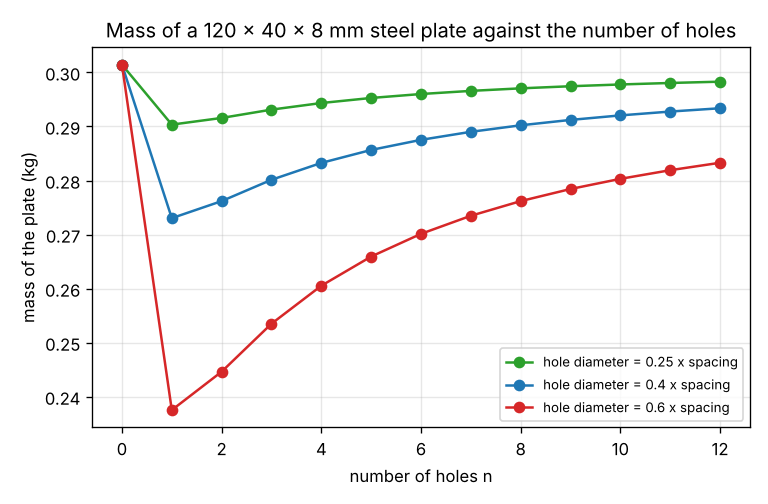
\includegraphics[width=0.78\textwidth]{figures/s01_mass_vs_holes.png}\caption{Mass of the plate against the number of holes, for three hole ratios.}\end{figure}

\begin{figure}[h]\centering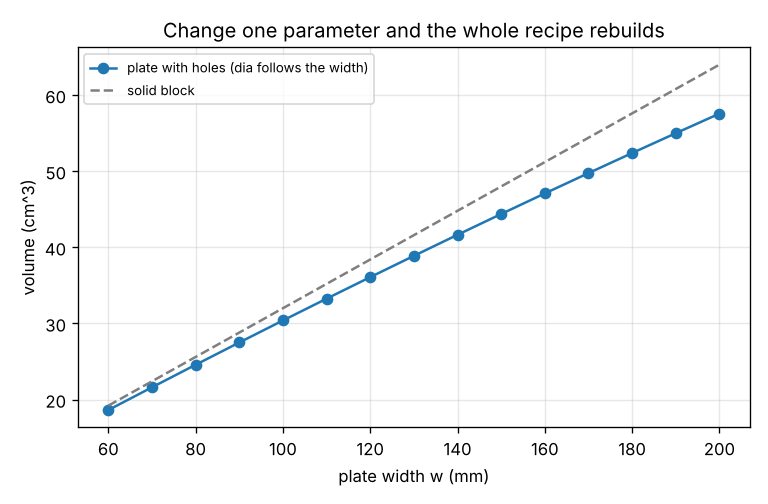
\includegraphics[width=0.78\textwidth]{figures/s01_volume_vs_width.png}\caption{Volume against the width: one parameter changes, the whole recipe rebuilds.}\end{figure}

\subsection*{E. Worked example}
\textbf{Problem.} The customer wants 6 holes instead of 4 and a width of 140 mm, with the same hole ratio of 0.4, depth 40 mm and thickness 8 mm. Find the spacing, the hole diameter, the volume and the mass of the new plate.

\begin{enumerate}[nosep]
\item Spacing: s = w / (n + 1) = 140 / 7 = 20.0 mm.
\item Diameter: dia = 0.4 x 20.0 = 8.0 mm. The holes fit: 8.0 is smaller than the spacing (20.0) and the depth (40).
\item Block: 140 x 40 x 8 = 44800 mm3.
\item Holes: 6 x (pi / 4) x 8.0\textasciicircum{}2 x 8 = 2413 mm3.
\item Volume: 44800 - 2413 = 42387 mm3, which is 42.39 cm3.
\item Mass: 7850 x 42387 x 1e-9 = 0.333 kg.
\end{enumerate}
\textbf{Answer.} The new plate has holes of 8.0 mm, 20.0 mm apart, a volume of 42.4 cm3 and a mass of 0.333 kg, compared with 0.283 kg for the original.

\section{Session 2: From an outline to the properties of a solid: area, centroid and stiffness}

\subsection*{A. Real-world problem}
A shelf bracket is cut from an L-shaped steel section. Two sections with the same mass can bend very differently under the same load. Which numbers of the outline decide how stiff it is, and how do we compute them from the corner points of a sketch? For an L of 50 x 50 x 5 mm carrying a bending moment of 100 N m, how large is the stress?

\subsection*{B. Concept and theory}
A sketch outline is a list of corner points joined by straight edges, and a hole is a circle. Three numbers describe how the area is spread. The area A is the amount of material. The centroid (Cx, Cy) is the balance point of the outline. The second moment of area Ixx = integral of y\textasciicircum{}2 dA, with y measured from the horizontal line through the centroid, measures how far the material lies from that line, squared. In bending, the stress at a distance c from the neutral axis is sigma = M c / Ixx, so for the same moment M a section with a larger Ixx has smaller stress and bends less. For corner points listed counter-clockwise, with cross\_i = x\_i y\_(i+1) - x\_(i+1) y\_i, the area is A = 1/2 sum cross\_i, and the centroid and the moments about the origin follow from similar sums (the formulas are in the lesson). A hole is a shape whose moments are subtracted. To move the second moment from the origin to the centroid we use the parallel-axis rule, Ixx = Ix0 - A Cy\textasciicircum{}2. An extruded section of length l has the volume A l and the mass rho A l. The key idea is that Ixx weights each piece of area by the square of its distance from the axis, so material far from the axis is far more useful than material near it.

\begin{itemize}[nosep]
\item A: area of the section (mm\textasciicircum{}2)
\item Cx, Cy: centroid of the section (mm)
\item Ixx, Iyy: second moment of area about the horizontal and vertical lines through the centroid (mm\textasciicircum{}4)
\item M: bending moment (N mm (1 N m = 1000 N mm))
\item c: distance from the neutral axis to the outer edge (mm)
\item sigma: bending stress, M c / Ixx (MPa (N/mm\textasciicircum{}2))
\item l: length of the extruded part (mm)
\end{itemize}

\[ A = \tfrac12\sum_i \left(x_i y_{i+1} - x_{i+1} y_i\right) \]

\[ I_{xx} = I_{x0} - A\,C_y^{2}\qquad\text{(parallel-axis rule)} \]

\[ \sigma = \frac{M\,c}{I_{xx}},\qquad m = \rho\,A\,\ell\cdot 10^{-9} \]

\subsection*{C. Visual explanation}
The first figure shows Ixx of a 50 x 50 mm L-section rising with its thickness t: a thin section is flexible and a thick one is stiff, but the curve also costs material. The second figure plots Ixx against the area, which is proportional to mass, for three heights of the vertical leg. At the same area, the taller leg is stiffer, because its material lies farther from the neutral axis.

\begin{figure}[h]\centering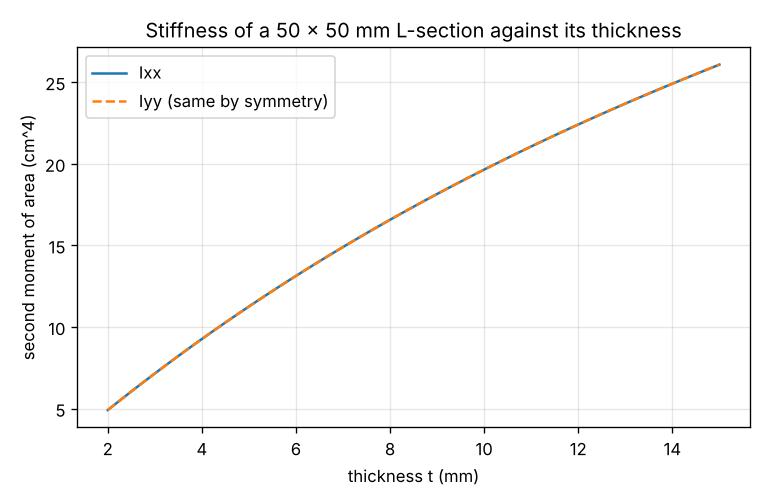
\includegraphics[width=0.78\textwidth]{figures/s02_ixx_vs_thickness.png}\caption{Ixx and Iyy of a 50 x 50 L-section against its thickness.}\end{figure}

\begin{figure}[h]\centering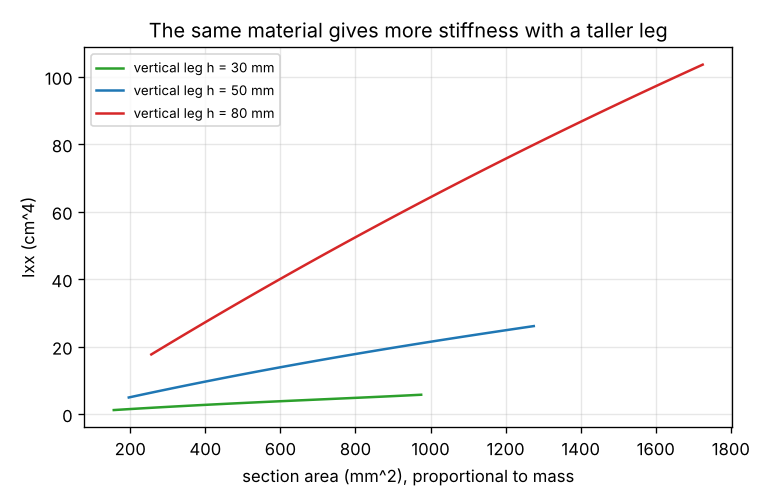
\includegraphics[width=0.78\textwidth]{figures/s02_ixx_vs_area.png}\caption{Ixx against the area for three leg heights: the same material, more stiffness.}\end{figure}

\subsection*{E. Worked example}
\textbf{Problem.} An L-section has a horizontal leg b = 60 mm, a vertical leg h = 40 mm and a thickness t = 10 mm. Find the area, the centroid, Ixx and Iyy, and the mass of a 300 mm length of steel.

\begin{enumerate}[nosep]
\item Split it into two rectangles: the horizontal leg 60 x 10 (area 600 mm2, centre (30, 5)) and the rest of the vertical leg 10 x 30 (area 300 mm2, centre (5, 25)).
\item Area: 600 + 300 = 900 mm2.
\item Centroid: Cx = (600 x 30 + 300 x 5) / 900 = 21.67 mm and Cy = (600 x 5 + 300 x 25) / 900 = 11.67 mm.
\item Ixx: 60 x 10\textasciicircum{}3 / 12 + 600 x (11.67 - 5)\textasciicircum{}2 + 10 x 30\textasciicircum{}3 / 12 + 300 x (25 - 11.67)\textasciicircum{}2 = 5000 + 26667 + 22500 + 53333 = 107500 mm4.
\item Iyy: 10 x 60\textasciicircum{}3 / 12 + 600 x (30 - 21.67)\textasciicircum{}2 + 30 x 10\textasciicircum{}3 / 12 + 300 x (21.67 - 5)\textasciicircum{}2 = 180000 + 41667 + 2500 + 83333 = 307500 mm4.
\item Mass: 7850 x 900 x 300 x 1e-9 = 2.12 kg. The lesson code, which uses the polygon sums, gives the same numbers.
\end{enumerate}
\textbf{Answer.} A = 900 mm2, centroid (21.67, 11.67) mm, Ixx = 107 500 mm4, Iyy = 307 500 mm4 and a mass of 2.12 kg for 300 mm.

\section{Session 3: How a sketch keeps its corners where you told it: a constraint solver}

\subsection*{A. Real-world problem}
In a CAD sketch you do not type coordinates. You say 'this line is horizontal, this one is 40 mm long, these two are perpendicular', and the program finds the corner points. When you change 40 to 60, the points move and the sketch stays consistent. How can a program find the points from such statements, know whether you have said enough, and notice when two statements contradict each other? What are the six corner points of an L-bracket of 50 x 50 x 5 mm, and how much does a 200 mm length weigh?

\subsection*{B. Concept and theory}
The unknowns are all the coordinates (x0, y0, x1, y1, ...). Each statement is turned into one or two residuals, numbers that are zero when the statement is true: 'point i is at (X, Y)' gives x\_i - X and y\_i - Y; 'points i and j are d apart' gives |p\_j - p\_i| - d; 'the line i-j is horizontal' gives y\_j - y\_i; 'vertical' gives x\_j - x\_i; and 'the angle i-j-k is 90 degrees' gives (p\_i - p\_j) . (p\_k - p\_j). We need the points where all residuals are zero together. Newton's method does this from a first guess x: compute the vector of residuals r and the Jacobian J, the table of how each residual changes with each coordinate; solve J dx = -r for the correction dx (least squares, which takes the smallest correction when there is freedom left); move x by dx and repeat until r is zero. A step that makes the residual worse is halved. The first guess matters because several sketches satisfy the same statements, for example a mirror image, and Newton's method finds the one near the guess. At the solution the rank of J counts the independent statements: degrees of freedom = 2 x (number of points) - rank(J). Zero means the sketch is fully constrained, more than zero means it can still be dragged. If there are more statements than the rank, some are redundant (fine if they agree), and if the residuals cannot be brought to zero the statements contradict each other.

\begin{itemize}[nosep]
\item x: all point coordinates in one list (x0, y0, x1, y1, ...) (mm)
\item r: vector of residuals, zero when the statements are true (mm)
\item J: Jacobian: change of each residual per change of each coordinate (no unit)
\item dx: Newton correction, found from J dx = -r (mm)
\item DOF: degrees of freedom = 2 (number of points) - rank(J) (no unit)
\item b, h, t: legs and thickness of the L-bracket (mm)
\end{itemize}

\[ \mathbf r(\mathbf x) = \mathbf 0,\qquad \mathbf r\ \text{from}\ x_i - X,\ \ |p_j - p_i| - d,\ \ y_j - y_i,\ \ x_j - x_i,\ \ (p_i - p_j)\cdot(p_k - p_j) \]

\[ J\,\Delta\mathbf x = -\mathbf r,\qquad \mathbf x \leftarrow \mathbf x + \Delta\mathbf x \]

\[ \mathrm{DOF} = 2n_{\text{points}} - \operatorname{rank}(J) \]

\subsection*{C. Visual explanation}
The first figure plots the mass of a 60 x 40 mm L-bracket, 200 mm long, for 27 thicknesses, each found by solving the sketch again from the previous solution. The second figure shows the same sketch for two thicknesses: the points move so that every length stays true, and the shape keeps its orientation.

\begin{figure}[h]\centering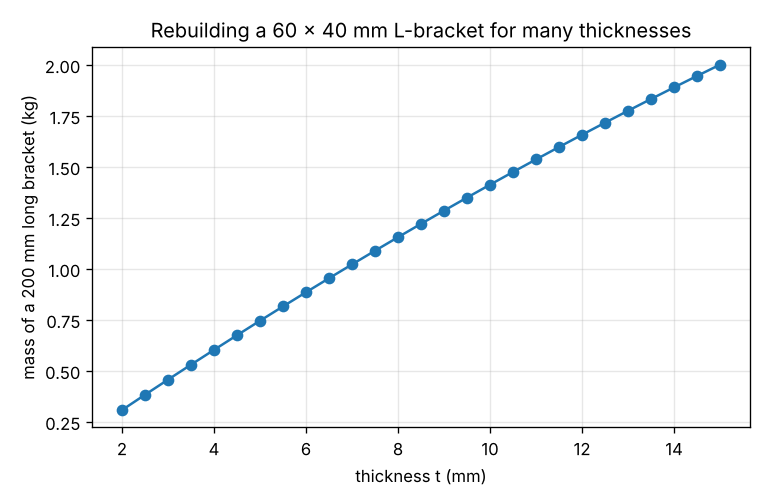
\includegraphics[width=0.78\textwidth]{figures/s03_bracket_mass_vs_t.png}\caption{Mass of a 200 mm long L-bracket against its thickness, rebuilt by the solver.}\end{figure}

\begin{figure}[h]\centering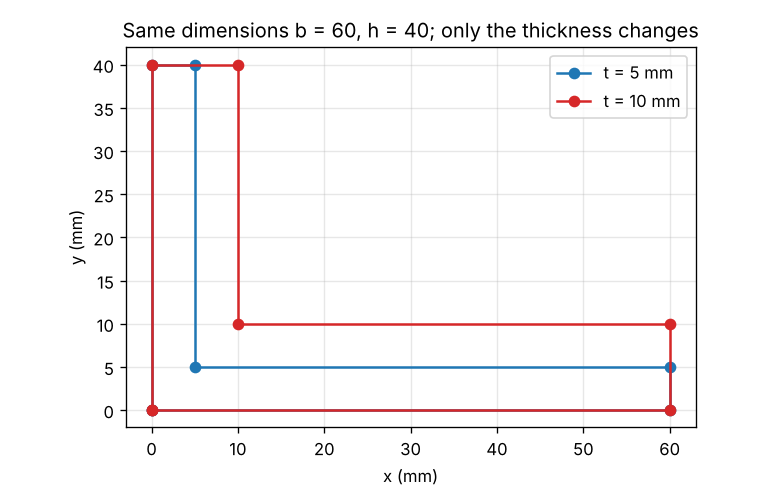
\includegraphics[width=0.78\textwidth]{figures/s03_sketch_rebuild.png}\caption{The same L-bracket sketch for two thicknesses.}\end{figure}

\subsection*{E. Worked example}
\textbf{Problem.} A triangle has one corner p0 fixed at the origin, p1 on the horizontal axis 4 mm from it, p2 at 3 mm from p0 and 5 mm from p1. Which statements does that make, and where are the points? Then find the area of the L-bracket 50 x 50 x 5 and its mass for 200 mm.

\begin{enumerate}[nosep]
\item Statements: fix p0 at (0, 0) (2 residuals), p0-p1 horizontal (1), |p0 p1| = 4 (1), |p0 p2| = 3 (1), |p1 p2| = 5 (1): six residuals for six coordinates, so the sketch can be fully constrained.
\item Newton's method from the rough guess (0, 0), (3, 0.5), (0.5, 2) converges in 4 steps to p1 = (4, 0) and p2 = (0, 3): the 3-4-5 triangle, with a right angle at p0 that we never asked for.
\item A guess with p2 below the axis gives the mirror image p2 = (0, -3): the guess chooses between valid sketches.
\item L-bracket: 6 points, 12 coordinates; p0 is fixed (2), five lines are horizontal or vertical (5) and five lengths are given (5): 12 equations, so DOF = 0. The solver gives [[0.0, -0.0], [50.0, -0.0], [50.0, 5.0], [5.0, 5.0], [5.0, 50.0], [0.0, 50.0]].
\item Area from the corner points by the shoelace formula: 475 mm2, equal to b t + (h - t) t = 250 + 225. Mass of 200 mm: 7850 x 475 x 200 x 1e-9 = 0.746 kg.
\end{enumerate}
\textbf{Answer.} The triangle is (0, 0), (4, 0), (0, 3); the L-bracket is fully constrained with area 475 mm2 and a mass of 0.746 kg for 200 mm.

\section*{Where to go next}
\begin{enumerate}[nosep]
\item \textbf{Arcs and circles in the sketch.} Add a circle (centre point and radius) and the statements 'radius is r', 'point on circle' and 'line tangent to circle' to the solver of Session 3.
\item \textbf{A feature tree with extrude, cut and revolve.} Extend the rebuild of Session 1 to a list of extrude, cut and revolve features, each with parameters, and recompute the volume after every change.
\item \textbf{Volume, centre of mass and inertia of a solid.} Add the centre of mass and the moment of inertia about an axis for extruded and revolved parts.
\item \textbf{Fillets and chamfers on the outline.} A function that replaces a convex corner of a polygon by a tangent arc and returns the new area and second moment of area.
\item \textbf{Assemblies and mates.} Give every part a position and an angle and solve the mates with the same Newton method as the sketch.
\end{enumerate}

This is a simplified educational model. It is not a validated design tool and must not be used for real structures, electrical installations, vehicles, industrial processes or medical decisions.

\end{document}
